\chapter{Stereo video watermarking}
\markright{Stereo video watermarking}
\label{wat}
\phantomsection
%\addcontentsline{toc}{chapter}{Stereoscopic Video}

\section{Watermaking}

Digital watermarking consists in imperceptiby and persistently associating some extra information with some original content. \\
The basic watermarking workflow is presented in Figure \ref{fig:workflow}.\\
\begin{figure}[h!]
\centering
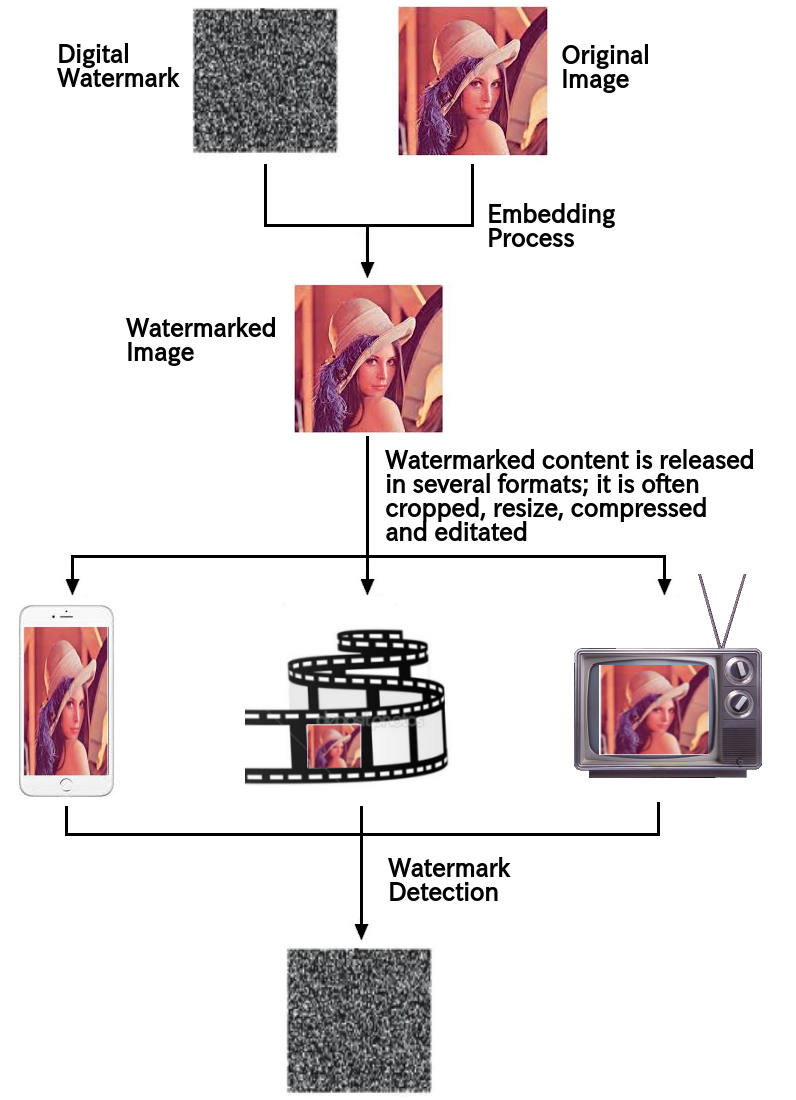
\includegraphics[width=0.6\textwidth]{./img/wat_workflow.png}
\caption{\small{Watermarking workflow}}
\label{fig:workflow}
\end{figure}
\clearpage
\subsection{Properties}
Three parameters are required to evaluate watermarking technique performances:
\begin{itemize}
\item[-] perceptual impact, that is the misure of how much the watermark affects the quality of the host data;
\item[-] robustness, i.e.,the capability of the hidden data to survive host signal manipulation including compression, signal processing, geometric manipulations;
\item[-] data payload, that is the amount of data of information bits that it is able to convey.
\end{itemize}
These requirements are though inversely proportional (Figure \ref{fig:properties}): the more information is embedded, the more the watermark is visible and viceversa; the more robusteness is encreased, the more the watermark is visible and viceversa.\\
\begin{figure}[h!]
\centering
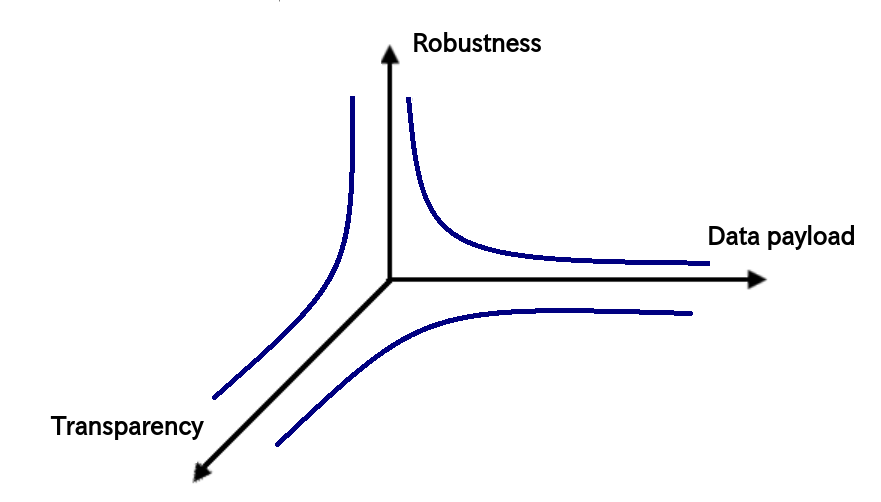
\includegraphics[width=0.4\textwidth]{./img/properties.png}
\caption{\small{Watermark properties trade-off}}
\label{fig:properties}
\end{figure}
Finally, a watermarking technique can be:
\begin{itemize}
\item[-] non-blind/blind, if at the decoder side the original content is available or not, respectively;
\item[-] private/public if only authorized users
can recover it or if anyone to read the watermark, respectively;
\item[-] detectable/readable, if it is only possible to decide whether a given watermark is embedded in the content or if the bits hidden in the content can be read without knowing them in advance, respectively.
\end{itemize}




\subsection{Embedding domains}
Host features modified during embedding can
belong to 
\begin{itemize}
\item[-] spatial domain: the watermark is embedded by directly modifying the pixel values;
\begin{figure}[h!]
\centering
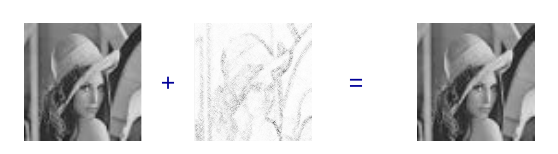
\includegraphics[width=1\textwidth]{./img/domain1.png}
\caption{\small{Spatial domain watermark insertion}}
\label{fig:dom1}
\end{figure}
\item[-] frequency domain: the image is transformed through a mathematical transformation, some coefficients are modified and finally the inverse transform is carried out;
\begin{figure}[h!]
\centering
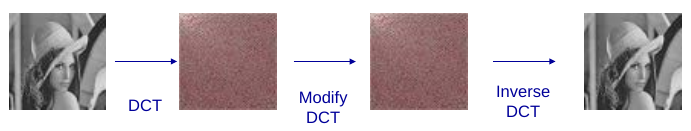
\includegraphics[width=1\textwidth]{./img/domain2.png}
\caption{\small{Frequency domain watermark insertion}}
\label{fig:dom2}
\end{figure}
\item[-] hybrid techniques: a block wise transform is applied, the image is divided
into blocks and for each block a mathematical transformation is computed, some coefficients are modified and the inverse transform is done.
\begin{figure}[h!]
\centering
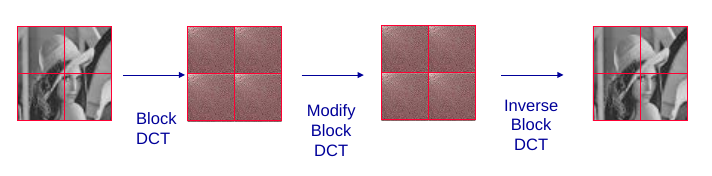
\includegraphics[width=1\textwidth]{./img/domain3.png}
\caption{\small{Hybrid technique}}
\label{fig:dom3}
\end{figure}
\end{itemize}

\subsection{Embedding techniques}
The most straightforward ways to add a watermark in a given content have been proved to be Spread Spectrum (SS) approach and Side Information (SI).\\
\begin{figure}[h!]
\centering
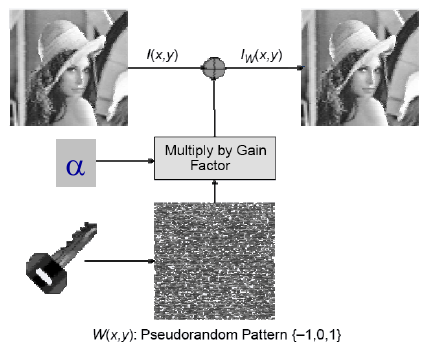
\includegraphics[width=0.6\textwidth]{./img/ss.png}
\caption{\small{Spread spectrum technique}}
\label{fig:ss}
\end{figure}
As in spread spectrum communications, the former approach considers the original content as a signal and the watermark as a noise that is spread over very many frequency bins so that the energy in any one bin is very small and certainly undetectable\cite{COX}\cite{COX1}.\\
The latter takes advantage of the fact that the original content is known at the embedder side (but unknown at the detector): this way the watermark can be modulated  according to the original and the quantity of inserted data can be maximed\cite{COX2,SH, EG, COSTA}.\\

Sometimes hybrid watermarking methods combining spread spectrum and side information concepts can be applied; they try to benefit from both the robustness and transparency of the spread spectrum methods and the increased data payload of the side information methods \cite{QIM}\cite{QIM1}.
\begin{figure}[h!]
\centering
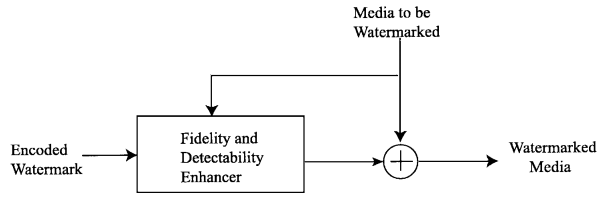
\includegraphics[width=0.7\textwidth]{./img/si.png}
\caption{\small{Side information technique scheme}}
\label{fig:si}
\end{figure}

\section{Stereoscopic video watermarking}

In the literature, stereoscopic video watermarking has been initially approached as a direct extension of still image watermarking, i.e. by considering the right and the left views as two independent images. This way, the stereo data can be straightforward exploited with basic 2D methods. However, such straightforward application does not consider the peculiarities of the stereoscopic video content, therefore a second modality considers derived representations from the stereo pair, as a disparity map.\\ 
A new approach, however, has been recently introduced in stereoscopic view-based methods: disparity-coherent watermarking \cite{DOER}.

\subsection{Embedding domain}
In stereoscopic video context the studies can be structured in two other categories in addition to spacial and frequency domain:
\begin{itemize}
\item[-] view-based methods \cite{16,17,18,19,20,21};
\item[-] disparity-based methods \cite{22}
\end{itemize}
according to the reference image in which the mark is actually inserted.\\
In Figure \ref{stereo_method} the workflows of both methods are presented.
\begin{figure}[h!]
\centering
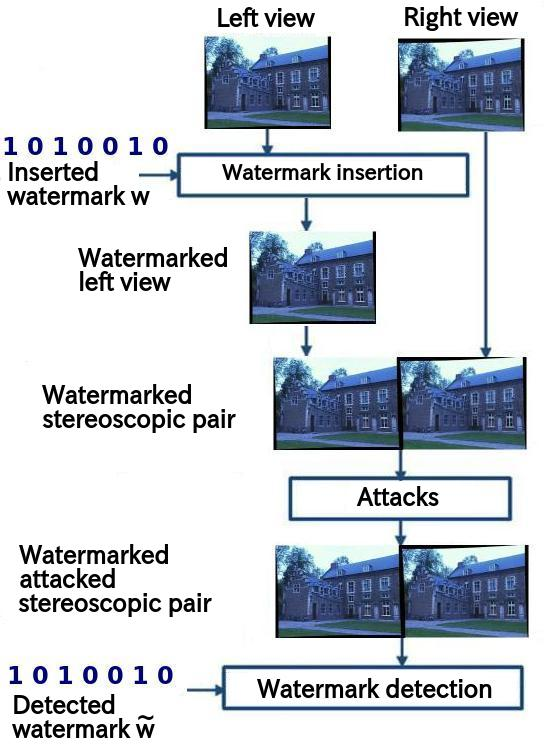
\includegraphics[width=0.8\textwidth]{./img/views_domain.jpeg}
\caption{\small{View-based watermarking workflow}}
\label{fig:view}
\end{figure}

\begin{figure}[h!]
\centering
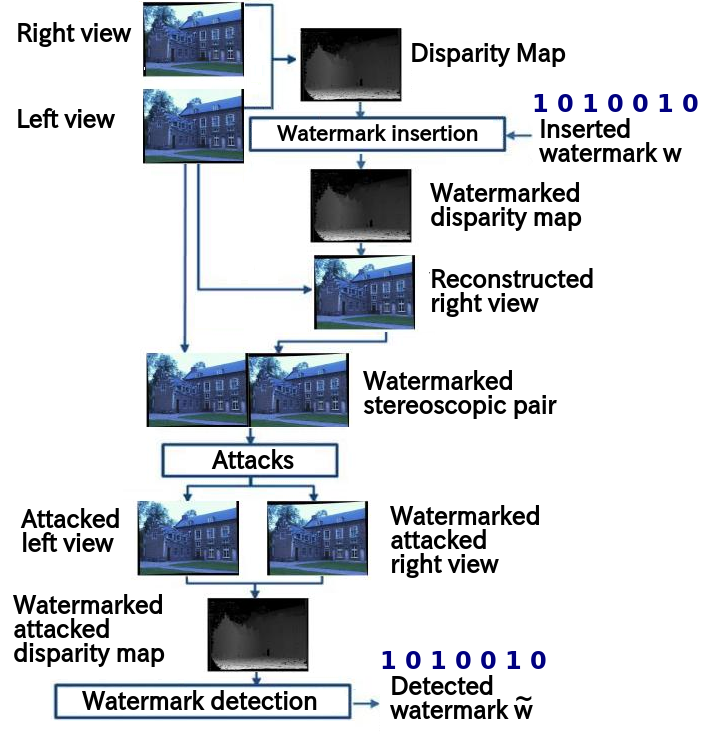
\includegraphics[width=1.05\textwidth]{./img/disparity_domain.png}
\caption{\small{Disparity-based watermarking workflow}}
\label{fig:disp}
\end{figure}


The predilection direction in the literature is represented by the view-based watermarking approaches, which are currently deployed for stereoscopic still images.\\ 
In this context disparity-coherent watermarking has been introduced,\cite{DOER}, to provide superior robustness against virtual view synthesis, as well as to improve perceived fidelity.\\
Disparity-coherence refers to the fact that a physical point of the captured scene should carry the
same watermark sample regardless of where it appears in the left/right view.\\
The advantages of producing disparity-coherent watermarks are two: first it produces pairs of stereoscopic views that are more in line with
what would naturally occur in reality and thereby yields less visual discomfort, second  disparity-coherent watermarks are expected to exhibit superior robustness against view synthesis, \cite{DOER}.\\
View synthesis consists in generating a virtual view in-between views that are available, e.g.the left and right views in stereo video. 

\subsection{Perception evaluation}

Perceptual impact can be defined as the imperceptibility of the embedded additional information in the watermarked content. This may signify either that the user is not disturbed by the artefacts induced by the watermark in the host document or that the user cannot identify any difference between the marked and the unmarked document.\\
The visual quality of the watermarked content in images and 2D video is usually objectively evaluated by five objective measures, namely, the PSNR, IF, NCC, SC, and SSIM \cite{METRICS}.\\

In this thesis the measures in \cite{QMETRICS} have been used to evaluate the quality of the watermarking technique in terms of human perception.\\
In Chaminda et al.'s study a Reduced-Reference
(RR) quality metric for color plus depth 3D video compression and transmission is proposed, using the extracted edge information of color plus depth map 3D video.\\ 
The work is motivated by the fact that the edges/contours of the depth map can represent different depth levels and this can be considered for measuring structural degradations. Since depth map boundaries are also coincident with the corresponding color image object boundaries, edge information of the color image and of the depth map is compared to obtain a quality index (structural degradation) for the corresponding color image sequence.\\
In order to quantify structural comparison, luminance comparison and contrast comparison parameters for the depth map and corresponding watermarked views, a modified version of the
commonly used SSIM metric is adopted:
\begin{equation}
Q_{Depth}(x,y) = [l(x,y)]^{\alpha} \cdot [c(x,y)]^{\beta} \cdot [\mathnormal{S}_{Depth}(x',y')]^{\gamma}
\end{equation}
where $l(x,y)$ and $c(x,y)$ are luminance and contrast comparisons performed on original depth maps and the ones computed after watermarking,
respectively, and $\mathnormal{S}_{Depth}(x',y')$  is the structural comparison between the gradient/edge maps of original and post-watermarking computed depth map images.\\
Then the overall depth map quality is calculated as
\begin{equation}
MQ_{Depth}(X,Y) = \frac{1}{M} \sum_{j=1}^{M}Q_{Depth}(x_{j},y_{j}).
\end{equation}
The SSIM-based quality index for the color image can be described as follows:
\begin{equation}
Q_{View}(x,y) = [l(x,y)]^{\alpha} \cdot [c(x,y)]^{\beta} \cdot [\mathnormal{S}_{View}(x',y')]^{\gamma}
\end{equation}
where $l(x,y)$ and $c(x,y)$ are luminance and contrast comparisons performed on original and watermarked views, respectively, and $\mathnormal{S}_{View}(x',y')$  is the structural comparison between the gradient/edge maps of the gradient maps of the corresponding original depth map and the watermarked views.\\
Hence, the overall color image quality is calculated as
\begin{equation}
MQ_{View}(X,Y) = \frac{1}{M} \sum_{j=1}^{M}Q_{View}(x_{j},y_{j}).
\end{equation}
As in \cite{QMETRICS}, the Sobel operator has been selected to obtain edge information (i.e., the binary edge mask) due to its simplicity and efficiency.\\

Finally the PSNR measure has been used to evaluate the quality of the watermarked videos and the quality of the compressed videos.\\
PSNR is the ratio between the maximum possible power of a signal and the power of corrupting noise that affects the fidelity of its representation; many signals have a very wide dynamic range, therefore PSNR is usually expressed in terms of the logarithmic decibel scale (dB). \\
For color images with three RGB values per pixel, the definition of PSNR is the following:
\begin{equation}
PSNR = 10 \cdot \log_{10}\bigg( \frac{MAX_{I}^2}{MSE}\bigg)
\end{equation}

\begin{equation}
MSE  = \frac{1}{3*MN} \sum_{i=0}^{M-1}\sum_{j=0}^{N-1}\Big(\mathbb{R} +\mathbb{G} + \mathbb{B}  \Big)
\end{equation}
with 
\begin{align}
\mathbb{R} &= [R_{I}(i,j)-R_{\tilde{I}}(i,j)]^{2} \\
\mathbb{G} &= [G_{I}(i,j)-G_{\tilde{I}}(i,j)]^{2} \\
\mathbb{B} &= [B_{I}(i,j)-B_{\tilde{I}}(i,j)]^{2}
\end{align}

where $I$ and $\tilde{I}$ are the $MxN$ reference image and the noisy approximation, respectively, and $MAX_{I}$ is the maximum possible pixel value of the image (when the pixels are represented using 8 bits per sample, this is 255).\\
For video sequence, the average value of all frames' PNSR value is computed.
Typical values for the PSNR in video compression and watermarking are between 30 and 50 dB.

\subsection{Robustness}
The robustness refers to the ability of detecting the watermark after applying some signal modifications
and malicious attacks on the marked content, such as spatial filtering, additive noise, geometric  transformations, lossy compression and, in stereoscopic context, view synthesis.

\subsubsection{Spatial filtering}
Linear filtering (such as blurring) and non-linear filtering (such as sharpening) are included in some image processing software: this operations remove from a signal some unwanted component or feature (Figure \ref{bl}).

\begin{figure}[h!]
\centering
\begin{subfigure}[]{0.4\textwidth}
\centering
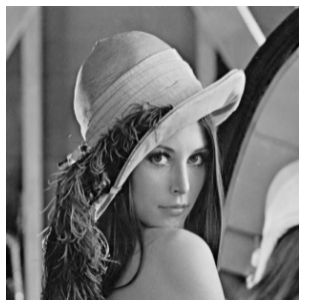
\includegraphics[width=0.8\textwidth]{./img/lena.png}
\caption{\small{Original image}}
\label{fig:lbO}
\end{subfigure}% 
\begin{subfigure}[]{0.4\textwidth}
\centering
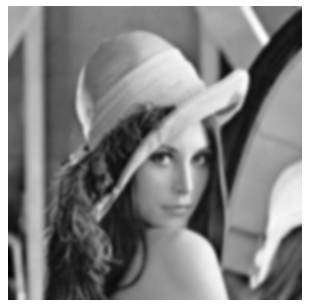
\includegraphics[width=0.8\textwidth]{./img/blur.png}
\caption{\small{Blurred image}}
\label{fig:blI}
\end{subfigure}% 
\caption{\small{Spatial filtering: blurring}\label{bl}}
\end{figure}

\subsubsection{Additive Noise}
The additive noise can be added to the content when applying some usual processing or when transmitting the signal over a communication channel during the broadcast (Figure \ref{noise}). 

\begin{figure}[h!]
\centering
\begin{subfigure}[]{0.4\textwidth}
\centering
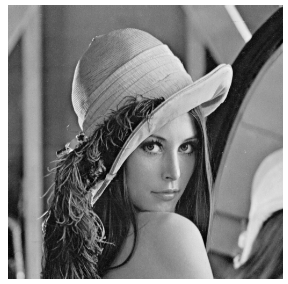
\includegraphics[width=0.8\textwidth]{./img/lena2.png}
\caption{\small{Original image}}
\label{fig:noise1}
\end{subfigure}% 
\begin{subfigure}[]{0.4\textwidth}
\centering
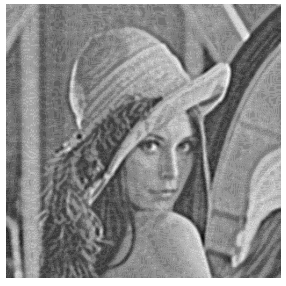
\includegraphics[width=0.8\textwidth]{./img/noise.png}
\caption{\small{Noised image}}
\label{fig:noise2}
\end{subfigure}% 
\caption{\small{Additive noise}\label{noise}}
\end{figure}

\subsubsection{Geometric distortions}
The geometric distortions include rotations, translations, spatial scaling, cropping and changes in aspect ratio (Figure \ref{geom}) they commonly occur during format changes.

\begin{figure}[h!]
\centering
\begin{subfigure}[]{0.4\textwidth}
\centering
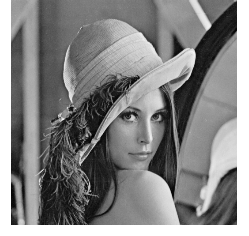
\includegraphics[width=0.8\textwidth]{./img/lena3.png}
\caption{\small{Original image}}
\label{fig:geom1}
\end{subfigure}% 
~ %add desired spacing between images, e. g. ~, \quad, \qquad,  etc.$  $
  %(or a blank line to force the subfigure onto a new line)
\begin{subfigure}[]{0.4\textwidth}
\centering
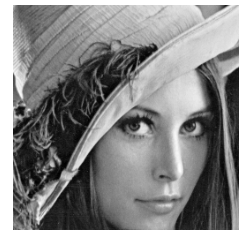
\includegraphics[width= 0.8\textwidth]{./img/crop.png}
\caption{\small{Cropped image}}
\label{fig:geom2}
  \end{subfigure}
\begin{subfigure}[]{0.4\textwidth}
\centering
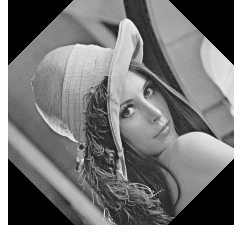
\includegraphics[width=0.8\textwidth]{./img/rot.png}
\caption{\small{Rotated image}}
\label{fig:geom3}
\end{subfigure}
\caption{\small{Geometric transformations}\label{geom}}
\end{figure}

\subsubsection{Lossy compression}
In video analysis, lossy compression is a common operation as it helps reduce resource usage, such as data storage space or transmission capacity.\newline  This process brings to a degradation of the image due to the compression ratio, thus affects the embedded watermark, as it removes the redundancy exploited in
watermarking schemes.\newline To prevent this problem a solution can be to improve the strenght of the embedded watermark.

\subsubsection{View synthesis}
Since in stereoscopic video context it is rather common practice to generate intermediate virtual views to adjust depth perception and since such view synthesis introduces non-rigid local geometric distortion that are not properly tackled by state-of-the art resynchronization mechanisms, stereo video watermarking strategies have to achieve robustness to synthetic view synthesis (Figure \ref{fig:vs}).\\

\begin{figure}[h!]
\centering
\begin{subfigure}[]{0.4\textwidth}
\centering
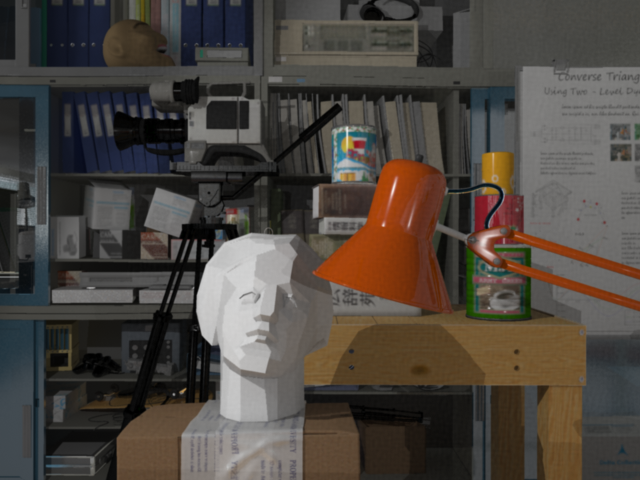
\includegraphics[width=0.8\textwidth]{./img/left_watermarked.png}
\caption{\small{Left image}}
\label{fig:vs1}
\end{subfigure}% 
~ %add desired spacing between images, e. g. ~, \quad, \qquad,  etc.$  $
  %(or a blank line to force the subfigure onto a new line)
\begin{subfigure}[]{0.4\textwidth}
\centering
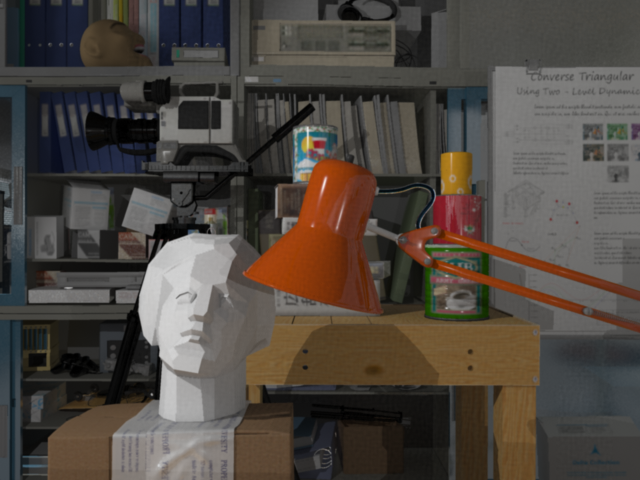
\includegraphics[width= 0.8\textwidth]{./img/right_watermarked.png}
\caption{\small{Right image}}
\label{fig:vs2}
  \end{subfigure}
\begin{subfigure}[]{0.4\textwidth}
\centering
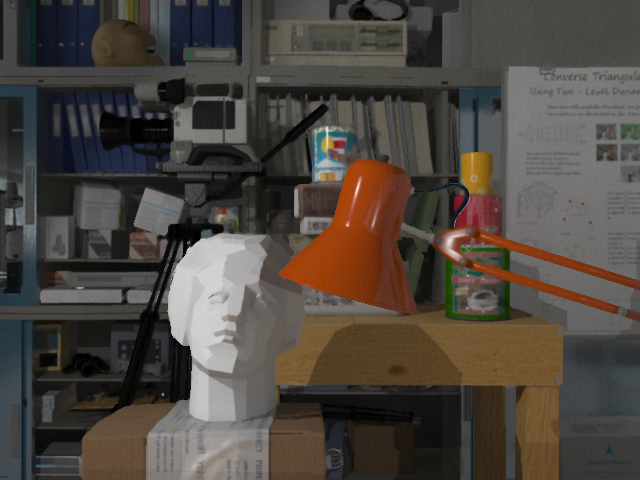
\includegraphics[width=0.8\textwidth]{./img/synth_view_watermarked.png}
\caption{\small{Synthetized view}}
\label{fig:vs3}
\end{subfigure}
\caption{\small{View synthesis}\label{fig:vs}}
\end{figure}



In this thesis a disparity-coherent watermarking algorithm has been implemented. It works in the frequency and spatial domain: a pseudo-random sequence of real numbers is embedded in a selected set of DFT coefficients of the left image then the reference watermark is spatially inserted in a disparity-coherent way in the right view.\\
It has shown good results in quality measure tests and roubustness test against view synthesis and compression.\\
An optimum criterion to verify if a given mark is present in an image is derived based on statistical decision theory, \cite{STAT}, allowing a robust watermark detection without resorting to the original uncorrupted image.\\







